\section{Ejemplo: Creación de un Blog}
Para ejemplificar, veremos la creación de un blog.

Las tareas a realizar son:
\begin{itemize}
\item Crear el modelo de clases.
\item Decidir cuales son las formas de interacción de los usuarios con el sistema.
\item Presentar esas formas de interacción de una manera atractiva y entendible para el usuario.
\end{itemize}

\section{Características del Modelo}

\subsection{Persistencia y metadata}
\label{sub-pers}

La persistencia del modelo se hace mediante la subclasificación de la clase especial \verb"PersistentObject".
Esta clase provee los métodos necesarios para describir la metadata en su inicialización, y también para las operaciones de guardado y borrado.

Para el blog, tendremos las siguientes clases: \emph{Post}, \emph{Tag}, \emph{User}.

\includegraphics*[scale=0.60,viewport=420 350 700 600]{diagrama.png}

\begin{verbatim}
class Post extends PersistentObject {
  function initialize() {
    $this->addField(new TextField(array('fieldName'=>'title')));
    $this->addField(new TextArea(array('fieldName'=>'text')));
    $this->addField(new CollectionField(
      array(
        'fieldName'=>'tags',
        'direct'=>false,
        'JoinType'=>PostTag,
        'targetField'=>'tag',
        'reverseField'=>'post')
       )
    );
    $this->addField(new IndexField(array('fieldName' => 'author', 'type' => 'User')));
  }
}

class PostTag extends PersistentObject {
  function initialize() {
    $this->addField(new IndexField(array('fieldName'=>'post', 'type' => 'Post')));
    $this->addField(new IndexField(array('fieldName'=>'tag', 'type' => 'Tag')));
  }
}

class Tag extends PersistentObject {
  function initialize() {
    $this->addField(new TextField(array('fieldName'=>'name')));
  }
}
\end{verbatim}

Esto define una clase persistente \verb"Post". En ella definimos un método initialize, en el que definimos los atributos que tiene un \verb"Post". En este caso son un \verb"título", un \verb"texto", una colección de \verb"etiquetas" y el usuario \verb"autor". La definición de un atributo se hace invocando el método \verb"addField" de \verb"PersistentObject" con el tipo de campo que queremos crear.

\subsection{Recuperación de objetos}
La recuperacion de objetos se hace mediante la clase \verb"Report", que permite obtener los objetos de una colección, filtrada por varios criterios y ordenada. Estos reportes tienen en cuenta las subclases de los objetos, y utilizan herencia para las variables de instancia.

\subsection{OQL (Object Query Language)}
\label{sub-oql}
Dada la complejidad de construir un reporte completo a mano, desarrollamos un lenguaje \emph{OQL} para consulta de los objetos, que construye un reporte. Desarrollar aquí la sintaxis y semántica del lenguaje sería muy largo y tedioso, por lo que presentamos un ejemplo de su utilización en el ámbito del blog que estamos desarrollando. Para obtener todos los \verb"Posts" cuya etiqueta sea una dada, agregamos en la clase \verb"Post":

\begin{verbatim}

class Post extends Component {
  ...
  function Tagged($tag){
    return #@select p:Post where exists (p.tags as tag where tag.name=$tag)@#;
  }
}

\end{verbatim}

La sintaxis extraña (los tokens \verb"#@" \verb"@#" que encierran la expresión de consulta) corresponde a la utilización de macros, que veremos en (sección \ref{sub-macros}).

Una buena propiedad del lenguaje es que está íntimamente relacionado con el código PHP, ya que puede utilizar las variables en el scope. Esta forma de implementación de lenguajes de dominio específico se denomina embebida.

\subsection{Adaptación de base de datos}
\label{sub-adapt}
\begin{figure}
	\centering 
	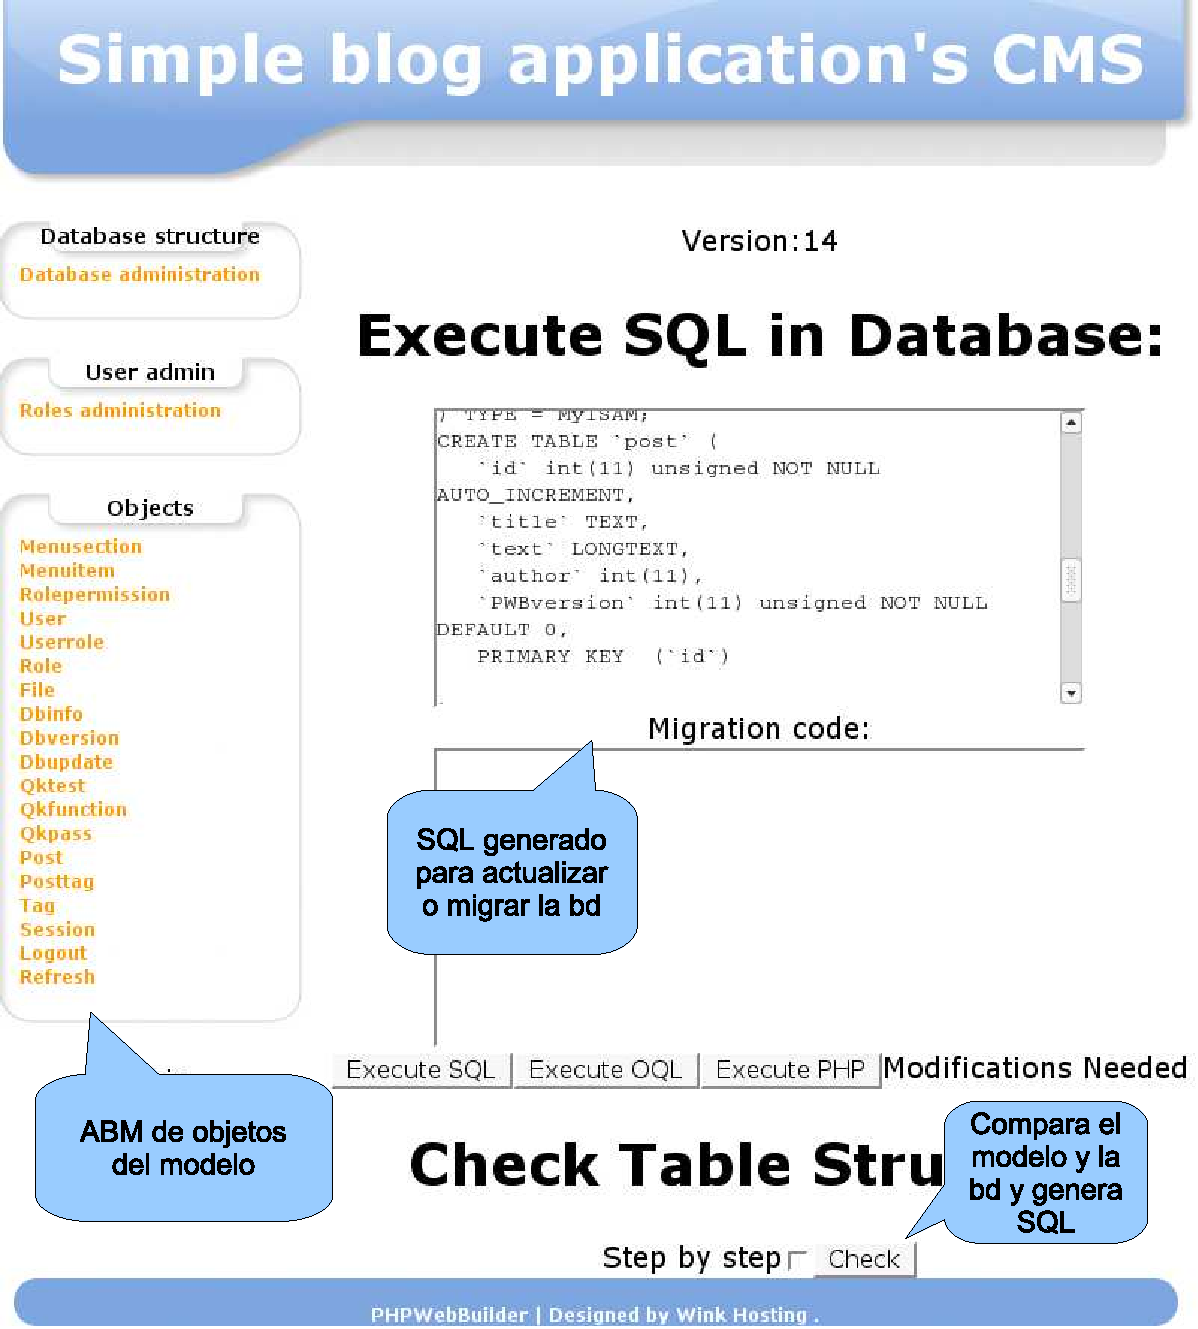
\includegraphics[scale=0.8]{admin2.eps} 
 	\caption{Adaptación de base de datos} 
 	\label{fig-admin1} 
\end{figure}

\begin{figure}
	\centering 
	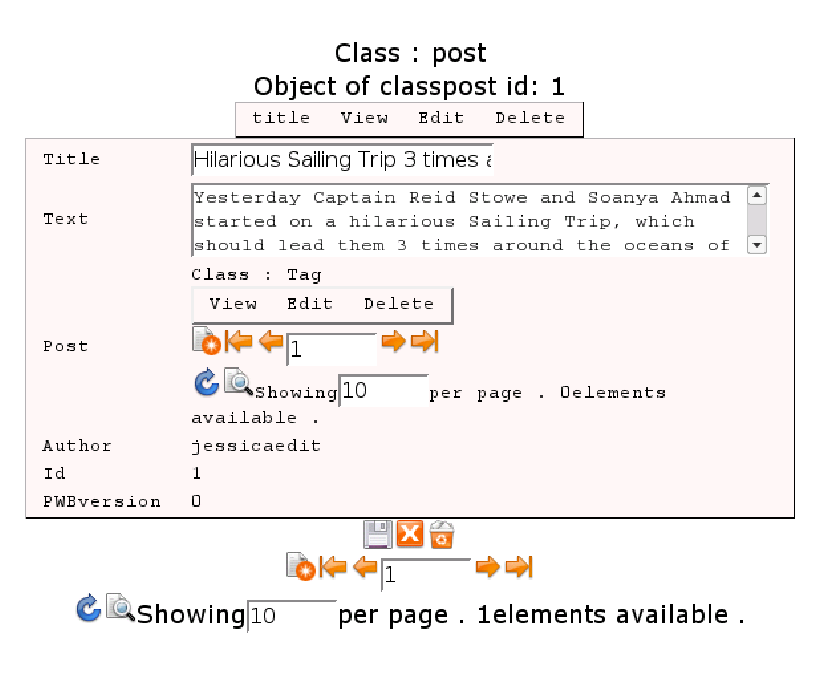
\includegraphics{abm1.eps} 
 	\caption{ABM Autogenerado de un Post} 
 	\label{fig-abm1} 
\end{figure}

\begin{figure}
	\centering 
	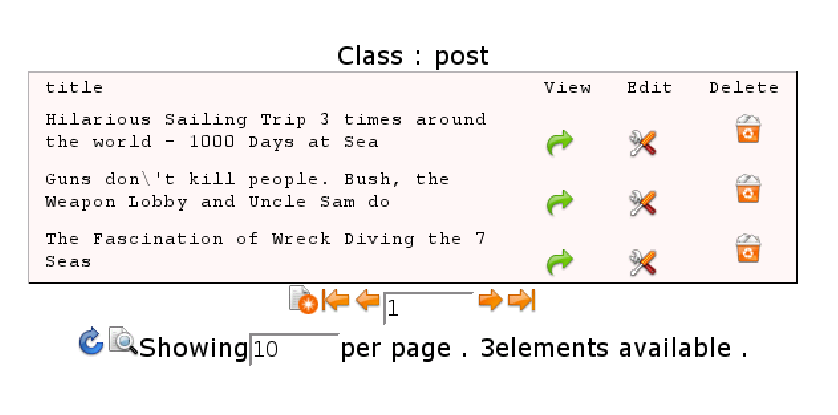
\includegraphics{abm2.eps} 
 	\caption{Aplicación de administración de Posts generada} 
 	\label{fig-abm2} 
\end{figure}

Los datos necesarios para la persistencia del modelo se infieren de la definición de los objetos. Establecemos los tipos de las variables de cada clase y las relaciones de subclasificación.

A partir de este modelo se puede deducir la información del esquema de persistencia para una base de datos relacional. \PWB \ genera el esquema automáticamente liberando de esta carga al programador, que es generalmente hasta más larga (y muchísimo más tediosa) que la programación del modelo.

Además, podemos verificar que el esquema de base de datos sea el correcto, y mostrar y ejecutar las correcciones necesarias. Esto también es muy útil cuando se hace una modificacion en el modelo de una aplicación y se necesita adaptar la base de datos a los nuevos cambios.
%Esta funcionalidad es provista por una herramienta que veremos más adelante.

\section{Características del Controller}
\label{sec-controller}
\subsection{Componentes}
\label{sub-comp}

Las aplicaciones se construyen mediante el ensamblado de componentes. Estos componentes son reutilizables, ya que pueden ser parametrizados, pueden disparar eventos, y pueden contener otros componentes.

Creemos el componente principal de la aplicación del blog. Este consiste simplemente de una lista de posts. Llamemos a este componente \verb"BlogComponent".

\begin{verbatim}

class BlogComponent extends Component {
  function initialize(){
      $this->addComponent(new PostList(#@select Post@#));
  }
}
\end{verbatim}

Como se ve en el ejemplo, un componente agrega sus sub-componentes definiendo un método \verb"initialize" e invocando a \verb"addComponent". Lo interesante de esta forma de diseñar la aplicación es que podemos obtener un componente a partir de otros componenentes ya implementados y probados. Además, cada componente posee su propio flujo de control. Esto significa que podemos componer libremente, casi sin restricciones y sin preocuparnos por formularios o pasaje de parámetros por URL, conceptos que surgen al desarrollar aplicaciones web en cualquier otro framework. Por último, cada componente maneja su propia entrada de datos y actualización de vistas.

Ahora definamos la lista de \verb"Posts". Sólo basta subclasificar de \verb"CollectionNavigator", un componente general para navegación y mostrado de listados de objetos:

\begin{verbatim}
class PostList extends CollectionNavigator {
  function addLine($post){
    return new PostItem($post);
  }
}

class PostItem extends Component {
  function PostItem($post){
    $this->post = $post;
    parent::Component();
  }

  function initialize(){
    $this->addComponent(new Text($this->post->title), 'title');
    $this->addComponent(new Text($this->post->text), 'text');
    // Mostramos las etiquetas del post
    $this->addComponent(new Component, 'tags');
    foreach($this->post->tags->collection->elements() as $tag){
      $this->tags->addComponent(new Text($tag->name));
    }
  }
}

\end{verbatim}

Un componente \verb"CollectionNavigator" presenta links para la navegación de los elementos (mostrandolos paginados). Para determinar cómo se van a manejar cada uno de los elementos se retorna un componente en el método \verb"addLine".

\subsection{Control de flujo modal}
\label{sub-modal-flow}
Veamos ahora otra característica del control de flujo de los componentes. Como vimos antes, cada componente posee su propio flujo de control lo que nos permitía ensamblar componentes más complejos libremente. Además de esto, la navegación a través de la aplicación se define mediante una interacción modal entre los componentes. Será mejor ver como funciona ésto en la aplicación que estamos desarrollando.

Queremos ahora poder ver la lista de \verb"Posts" filtrada por los que tienen una determinada etiqueta al hacer click sobre ésta. Reveamos entonces nuestras clases \verb"PostItem" y \verb"PostList" para establecer la interacción necesaria.

Modificamos primero la clase \verb"PostItem" para convertir las etiquetas mostradas a links. Para esto agregamos widgets de clase \verb"CommandLink" en lugar de los de clase \verb"Text" anteriores. Queremos actuar cuando una etiqueta es seleccionada, por lo tanto indicamos que el componente contenedor sea notificado mediante la invocación del método \verb"tagSelected" a través de la creación de un \verb"FunctionObject". Cuando una etiqueta es seleccionada, el \verb"PostItem" avisa disparando  un evento \verb"tag_selected".

\begin{verbatim}

class PostItem extends Component {
  function PostItem($post){
    $this->post = $post;
    parent::Component();
  }
  function initialize(){
    $this->addComponent(new Text($this->post->titulo), 'title');
    $this->addComponent(new Text($this->post->texto), 'text');
    // Mostramos las etiquetas del post
    $this->addComponent(new Component, 'tags');
    foreach($this->post->tags->collection->elements() as $tag){
      $this->tags->addComponent(new CommandLink(array('text'=>$tag->name,
        'prodeedFunction'=> new FunctionObject($this, 'tagSelected', array('tag'=>$tag)))));
    }
  }

  function tagSelected($params) {
    $this->getParent()->showTag($params);
  }
}

\end{verbatim}

Ahora falta que lista de \verb"Posts" se entere de que una etiqueta fue seleccionada y actuar en consecuencia. Modifiquemos la clase \verb"PostList" para que delegue su comportamiento a otra lista cuyos \verb"Posts" son sólo aquellos que poseen la etiqueta seleccionada. Registramos interés en el evento para que cuando sea disparado la lista principal delegue el control a la nueva lista filtrada como aparece en la implementación de \verb"showTag". La delegación de control se logra mediante la invocación del método \verb"call". Desde el punto de vista de la vista, la delegación de control implica que el componente llamante reemplazará su vista por la del componente llamado.

\begin{verbatim}

class PostList extends CollectionNavigator {
  function addLine($post){
    return new PostItem($post);
  }
  function showTag($params){
    $this->call(new PostList(Post::Tagged($params['tag']));
  }
}

\end{verbatim}


%Falta explicar la forma que tiene un componente de decir que terminó con su tarea. Hacemos esto invocando al método callback sobre el componente que terminó su ejecución.

%En el caso del PostList, una vez que se haya seleccionado una de sus etiquetas, su ejecución acaba y por lo tanto indica esto haciendo callback y pasando la etiqueta seleccionada al llamador.


%En el método \verb"showTag" del \verb"PostList", el componente llama (\verb"call") a otro componente, para realizar una tarea complementaria (en este caso, mostrar una lista distinta de posts, sólo aquellos que tienen el tag correspondiente).

\subsection{Widgets}
\label{sub-widget}

Existen unos componentes especiales, llamados \verb"Widgets"\cite{WDGTS}, que permiten interactuar con el usuario (por ejemplo con el componente \verb"Input", que permite recibir un string del usuario, el \verb"Text", que le presenta un texto, o el \verb"CheckBox", que presenta un checkbox).

Un \verb"Widget" especial, es el \verb"CommandLink", que permite al usuario ejecutar una acción en la aplicación como vimos en la sección \ref{sub-modal-flow}

% \subsection{Multiple Dispatching y Context Dispatching}
% \label{sub-dispatch}
% Otra característica llamativa, es el múltiple dispatching de funciones.
% Dado que muchas veces el método a utilizar depende de más de una clase, las funciones de múltiple dispatching nos ayudan a resolver este problema.
%
% Primero se define la función, con los parametros a utilizar tipados, y luego se hace el llamado, que utiliza los tipos de los parámetros para resolver el método a utilizar
%
% Además, las funciones de múltiple dispatching pueden ser utilizadas pasando el contexto (la rama de componentes dentro de la que se hace el llamado) de aplicación, para de esta manera poder responder de manera diferente a un evento, dependiendo del contexto.
%
% Por ejemplo, podemos tener un componente TaskList que muestre las tareas realizada en un día. Para cada tarea muestra la descripción, la hora, y el nombre de quién la completo en un componente TaskList. Si luego quisieramos ver las tareas realizadas por uno de los usuarios, nos interesaría ver la hora, la descripción, pero no el nombre del usuario, porque ya se sabe por el contexto. Podríamos usar en ese caso un componente UserTaskShow.
%
% Para implementar esa diferencia, una forma común sería tener 2 componentes, TaskList y UserTaskList. Esto duplica código, y además es difícil de implementar cuando el contexto de los componentes es de varios componentes (ya que tendríamos que hacer un nuevo componente para cada elemento en la rama de componentes hasta llegar al que realmente implementa la diferencia).
%
% Entonces, podemos utilizar el Context Dispatching para elegir un componente UserTaskShow, en lugar del otro, el TaskShow, independientemente del nivel de anidamiento del componente que hace el dispatch y el componente que provee el contexto.


\section{Características de la Vista}
\label{sec-view}
\subsection{Templates}
\label{sub-templates}
Para la generación de interfaz, utilizamos la técnica conocida de los templates.

\begin{verbatim}

<templates>
  <template class="PostItem">
    <h1><container id="titulo"/></h1>
    <p><container id="texto"/></p>
    Tags: <div id="tags"><container class="CommandLink"/> </div>
    <hr/>
  </template>
</templates>

\end{verbatim}

Por comodidad, agregamos las siguientes características:

- Los templates se ``heredan'', así que un Componente subclase de otro que tiene template, hereda de este el template (siempre y cuando no tenga uno más específico). También son heredables por \verb"Mixins" (sección \ref{sub-mixins}).

- Los templates son declarativos: No incluyen comandos ni iteradores (como tienen otros engines de templates). De esta manera, el control de la aplicación está 100\% en los componentes, y además nos aseguramos que los templates generen un XML bien formado.

- Los templates están basados en XML, con un par de tags extras (\verb"<template>" y \verb"<container>"), así que se puede generar cualquier XML (como XHTML) para mostrar los componentes.

Además, cada componente tiene un template default, por lo que no se necesita crearle uno para tener la aplicación funcionando (en nuestro caso, no lo hicimos para el \verb"BlogComponent" ni el \verb"PostList").

\subsubsection{Adaptación de Diseños existentes}
\label{sub-templates-adapt}
Debido a que los templates son XML, se puede tomar una página en HTML y agregarle los tags \verb"<template>" y \verb"<container>" donde se quiera, y de esta manera conseguir un template a muy bajo costo. Además, como los templates se heredan, utilizando \verb"Mixins" (sección \ref{sub-mixins}) y subclases, una aplicación puede tener un diseño completo en solo 3 o 4 templates.

\subsection{Renderings}
\label{sub-render}
El rendereo (generación de la interfaz) de la aplicación se hace 100\% mediante \PWB, de modo que no necesita nigún trabajo especial por el programador.

La manera de cambiar el engine de rendereo es tan simple como cambiar en el archivo de configuración, donde dice \verb"page_renderer=StandardPageRenderer" por \verb"page_renderer=AjaxPageRenderer", o incluso por \verb"page_renderer=CometPageRenderer" o \verb"page_renderer=XULPageRenderer".

\subsubsection{AJAX y Comet}

Todo lo generado por \PWB \ es XML bien formado, de modo que de manera transparente podemos renderear en AJAX.

Comet es una tecnología similar a AJAX, que se caracteriza por mantener una conexión abierta entre el browser y el servidor en todo momento. \PWB \ aprovecha esto, ya que un importante tiempo de procesamiento de los scripts PHP es la carga del script y los datos de la sesión de usuario, que en este caso quedan vivos en la memoria del servidor.

Mediante pasaje de mensajes de otro script, que envía los datos a la aplicación \PWB \ ejecutándose, podemos mantener la sesión en memoria, mejorando los tiempos de respuesta, e incluso modificando la aplicación del usuario no solamente cuando éste genera un evento (ej: un click del mouse), sino también cuando, por ejemplo, la base de datos es modificada.

\subsubsection{XUL}

El proyecto Mozilla incluye un subproyecto llamado XUL\cite{XUL}. XUL es un lenguaje de definición de interfaces desktop en XML. Dado que la salida de la aplicación debe ser un XML bien formado, y que la interacción usuario-interfaz se hace mediante javascript, \PWB \ soporta un XUL Page Renderer, que renderea aplicaciones en XUL. La diferencia para el programador, es en los tags de los templates, ya que debe utilizar elementos XUL en lugar de HTML. Dado que los templates de HTML llevan extensión .xml, y los de xul .xul, la misma aplicación, con tener templates de los 2 tipos para cada componente, puede ser rendereada de las 2 maneras.

\section{Características de \PITS}

\subsection{BugNotifier}

\PWB \ incluye un \verb"BugNotifier", que automatiza el manejo de errores ``no manejados'' , permitiendo al usuario que encuentra una condición de error dentro de la aplicación, enviar el reporte de error a un mail configurado a tal fin, y también reiniciar la aplicación para continuar utilizándola.

%En caso de que en la aplicación de Blog se encuentre un error, en lugar de presentarle al error, se le presentará con esta imagen.

\subsection{Eventos}
\label{sub-events}
\PWB \ implementa un mecanismo simple de eventos. Todo objeto \verb"PWBObject" implementa los mensajes \verb"addInterestIn", que permite a otro objeto escuchar un evento, y \verb"triggerEvent", que dispara un evento.

En nuestra implementación, el \verb"PostItem" tiene un \verb"CommandLink" que le envía a su componente padre el mensaje \verb"showTag". Esto trae problemas de composicionalidad, ya que no podríamos usarlo como hijo de un componente que no entienda ese mensaje.

% Hacer un diagrama representando esto.


Utilizando eventos, podríamos implementar:

\begin{verbatim}
class PostList extends CollectionNavigator{
  function addLine($post){
    $pi = new PostItem($post);
    $pi->addInterestIn('tagSelected', new FunctionObject($this, 'showTag'));
    return $pi;
  }
  ...
}

class PostItem extends Component{
  function initialize(){
    ...
    foreach($this->post->tags->collection->elements() as $tag){
      $this->tags->addComponent(new CommandLink(array('text'=>$tag->nombre,
        'prodeedFunction'=>new FunctionObject($this, 'showTag', array('tag'=>$tag))));
    }
  }
  function showTag($params){
    $this->triggerEvent('tagSelected', $params);
  }
}

\end{verbatim}

Existen objetos que accionan algunos eventos por default:
\begin{itemize}
\item Los \verb"Widgets", en cada acción del usuario (cuando hace click, cuando se modifica un elemento).
\item Los objetos del modelo (\verb"PersistentObject"), cuando son modificados.
\end{itemize}
%Por ejemplo, podríamos mostrar y ocultar el texto del post cuando se hace click en el título.

\subsection{Weak References}
\label{sub-weak}
Cuando un objeto \verb"$x" queda escuchando un evento de un \verb"PWBObject" \verb"$y", este último necesita guardar una referencia al primero. En caso de que, por el flujo de la aplicación, \verb'$x' deje de ser necesario, el mecanismo de garbage collection de PHP no puede descartarlo, porque \verb'$y' lo conserva referenciado, aunque no lo necesite realmente.

Por esto implementamos un mecanismo de Weak References, en donde \verb"$y" se queda con una referencia de \verb"$x", pero de la cual el garbage collector no se entera, permitiendo borrar a \verb"$x" en caso de que sea necesario.
 %$

\subsection{PHPCC}
\label{sub-phpcc}
Para crear el lenguaje OQL, debimos crear un Compiler Compiler para PHP (otros conocidos son Bison\cite{BISON}, yacc\cite{YACC}).
De esta manera ahora también se puede extender el framework con múltiples DSLs (Domain-Specific Languages - Lenguages específicos de Dominio).

\subsection{Macros}
\label{sub-macros}
Otra funcionalidad interesante, es la utilización de macros. Como se ve en lenguajes como C, las macros pueden llegar a tener un rol muy importante en un proyecto, ya que son otra forma de modularización.

Dentro de \PWB \ mismo, tenemos varios tipos de macros:

Las macros \verb"lam", y \verb"select", que permiten hacer un pre-procesamiento del código, generando código PHP con mayor funcionalidad:

\verb"#@select p:Post where exists (p.tags as tag where tag.nombre='Software Libre')@#"%$

genera un objeto reporte completo, con todos los posts con nombre \verb"'Software Libre'", en código PHP.

Y por otro lado, las macros para validación de código, que hacen tests, útiles para el momento del desarrollo pero consumidoras de tiempo valioso en tiempo de deployment.

Estas son typecheck, y check:
\verb"#@typecheck $p: Post@#" %$
que chequea que la variable \verb"$c" y %$
 sea un Post. En las opciones de configuración de la aplicación, habilitamos o dehabilitamos el typechecking, y el chequeo no se incluye.
\begin{verbatim}

class PostItem extends Component{
  function PostItem($post){
    #@typecheck $post: Post@#
    $this->post=&$post;
    parent::Component();
  }
  ...
}
\end{verbatim}

Esto detecta problemas durante el desarrollo, al intentar inicializar erróneamente un \verb"PostItem". Cuando la aplicación se instala en el cliente, se elimina el chequeo para evitar el overhead.

Un programador puede agregar sus propias macros, declarando una función \verb"mi_macro", y luego llamandola con \verb"#@mi_macro" {\it parámetros} \verb"@#".

\subsection{Mixins}
\label{sub-mixins}
Otra funcionalidad interesante es una implementación limitada de \verb"Mixins" (mediante \verb"Macros").

Un \verb"Mixin" es una forma de agrupar funcionalidad y agregársela a múltiples clases de objetos, sin que estas clases estén conectadas por subclasificación. Es lo que vemos como el mejor trade-off entre simple y múltiple herencia.

\begin{verbatim}
#@mixin ValueHolder {
  var $value;
  function getValue(){
    return $this->value;
  }
  function setValue($value){
    $this->value = $value;
  }
}@#

class Contador{
  #@use_mixin ValueHolder@#
  function increment(){
    $this->setValue($this->getValue()+1);
  }
}

class Direccion extends PersistentObject{
  #@use_mixin ValueHolder@#
  function initialize(){
    $this->addField(new TextField(array('fieldName'=>'value')));
  }
}

\end{verbatim}

De esta manera, podemos implementar una sola vez el comportamiento de \verb'ValueHolder', y utilizarlo en 2 clases distintas (\verb"Direccion" y \verb"Contador"), sin necesidad de relacionarlos por herencia.

Además, agregamos a los mixins en el chequeo de tipos. Si tenemos un \\ chequeo \verb"#@typecheck $v: ValueHolder@#", tanto un objeto de clase \verb"Direccion" como uno de clase \verb"Contador" cumplen con la condición.

\subsection{Múltiples Configuraciones}

Para el desarrollo colaborativo, es útil mantener múltiples configuraciones. O para trabajar en distintos clientes. O para hacer testing y deployment.

Por todo esto, \PWB \ mantiene un archivo de configuraciones múltiples, para adaptar cada una a una necesidad específica. En un archivo de configuración global (config.php) se guardan las variables específicas de cada configuración, además de las variables comunes a todas. Luego, en otro archivo (serverconfig) se pone la configuración que se va a utilizar.

\subsection{Compilación}

El uso de macros, y la inclusión de los muchos archivos de \PWB, hacen que la carga en cada request pueda ser muy lenta. Por eso implementamos una mini-compilación de los archivos PHP (para que las macros ya estén procesadas), y además, habilitamos varios outputs de esta compilación del código (todo a un sólo archivo PHP, sólo las clases utilizadas a un archivo PHP, en archivos separados). Esta configuración es seteable desde los archivos de configuración.